\chapter{Exploiting Software Diversification for \Wasm}
\label{exploit}

In this chapter ... 

\msection{Offensive Diversification: Malware evasion}

\todo{Motivate the use case with the following sota}

\wrule{Binary rewriting tools and obfuscators} The landscape for tools that can modify, obfuscate, or enhance \Wasm binaries for various has increased. 
For instance, BREWasm\cite{BREWasm} provides a comprehensive static binary rewriting framework specifically designed for \Wasm. 
Wobfuscator\cite{wobfuscator} takes a different approach, serving as an opportunistic obfuscator for Wasm-JS browser applications. 
Madvex\cite{madvex} focuses on modifying \Wasm binaries to evade malware detection, with its approach being limited to alterations in the code section of a \Wasm binary. 
Additionally, WASMixer\cite{wasmixer} obfuscates WebAssembly binaries, by including memory access encryption, control flow flattening, and the insertion of opaque predicates.


\todo{ The malware evasion paper}

\msubsection{Threat model and objective}

\begin{figure}
    \centering
    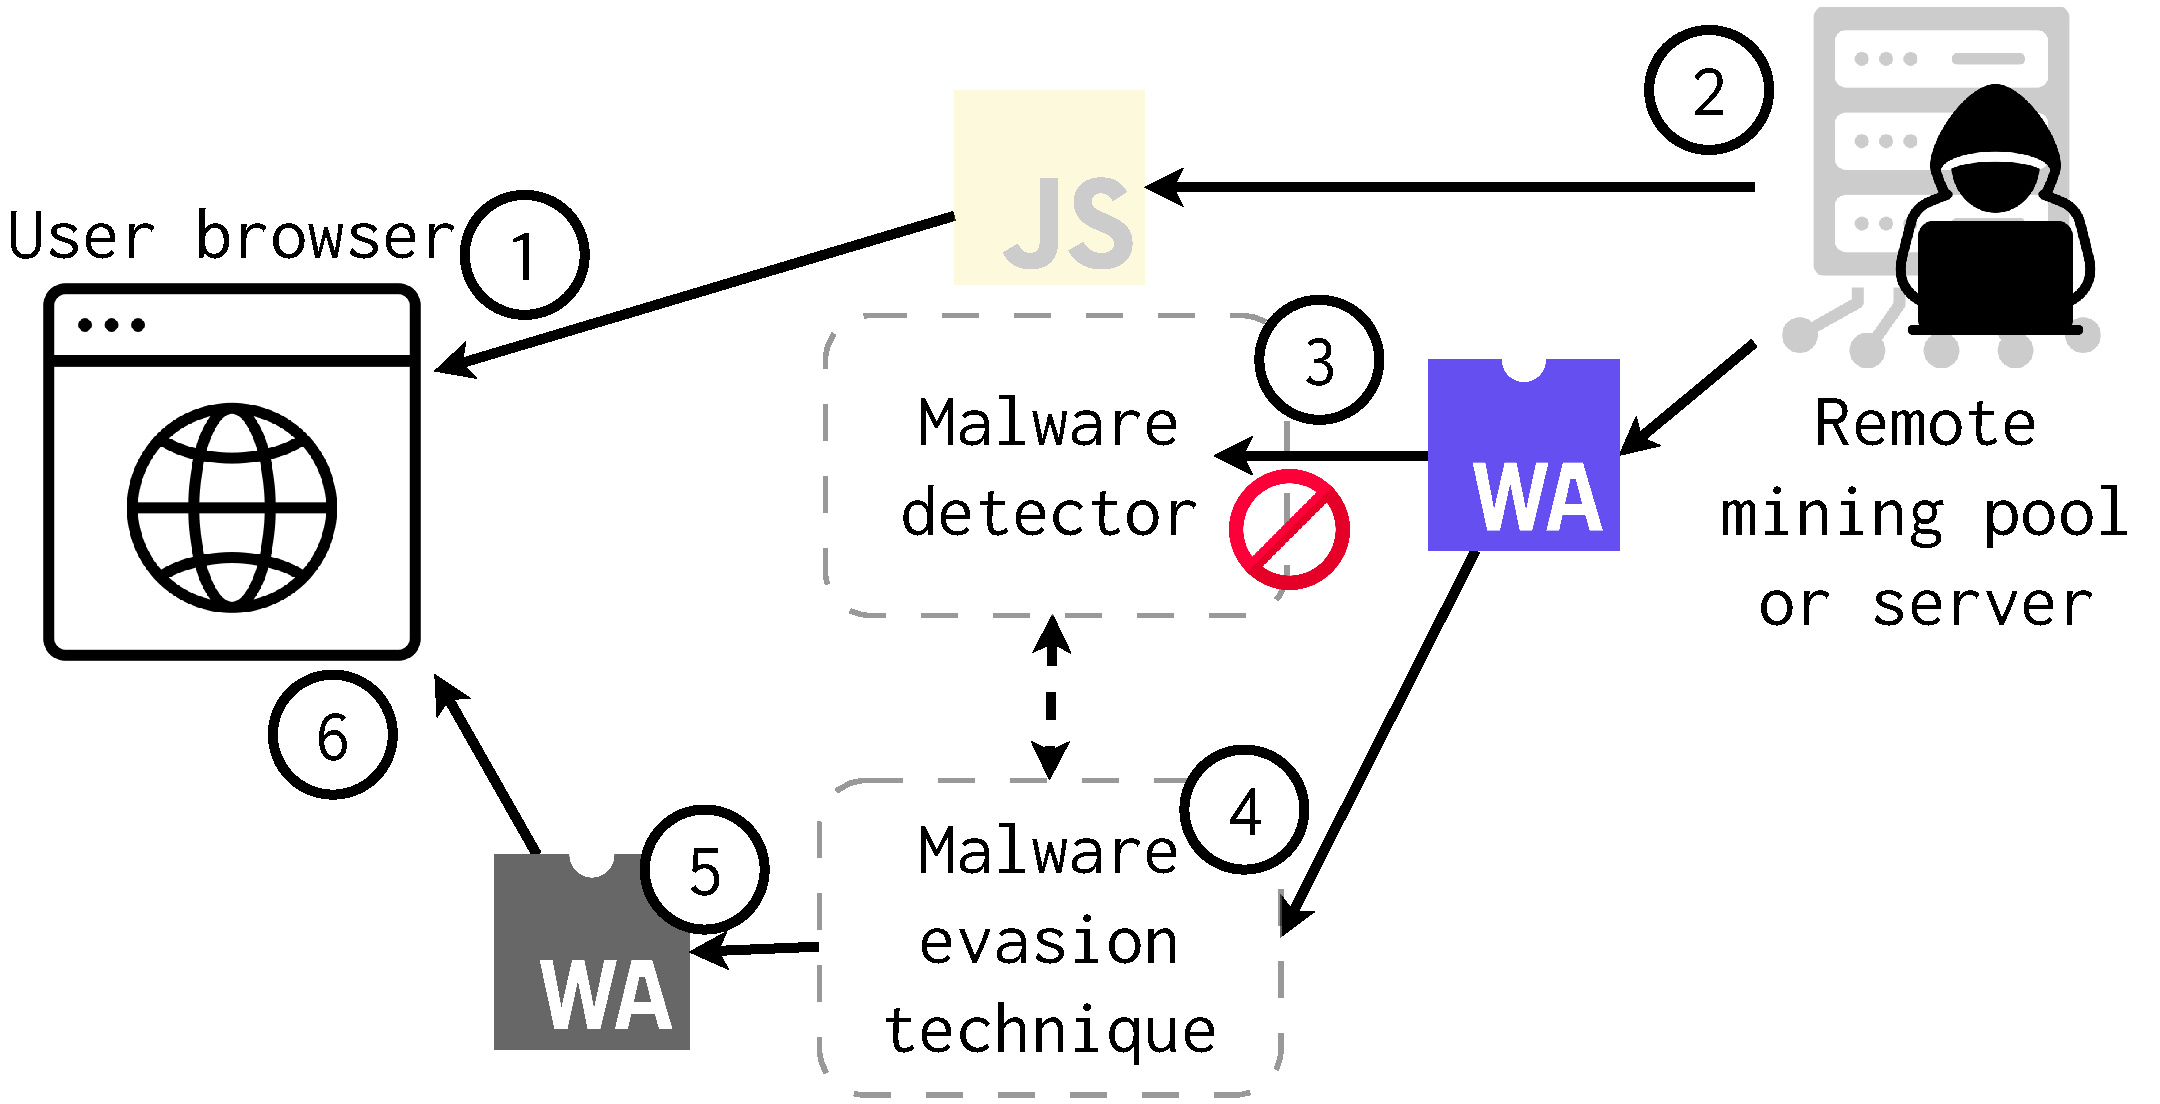
\includegraphics[width=0.8\linewidth]{figures/threat_model.pdf}
    \caption{Taken from \cite{EVASION}}
    \label{fig:threat_model}
\end{figure}

Test and evade the resilience of \Wasm malware detectors mentioned in \autoref{background:wasm:ecosystems}.


\msubsection{Approach}

%\lipsum[1]

\todo{We use wasm-mutate}
\todo{How do we use it?}
\todo{Controlled and uncontrolled diversification.}

%\lipsum[1]

%\lipsum[1]

\msubsection{Results}


\begin{tcolorbox}[title=Contribution paper,boxrule=1pt,arc=.2em,boxsep=1.0mm]
    The case discussed in this section is fully detailed in Cabrera-Arteaga \etal "WebAssembly Diversification for Malware Evasion"
    \emph{at Computers \& Security, 2023}
    \url{https://www.sciencedirect.com/science/article/pii/S0167404823002067}. 
\end{tcolorbox}

\msection{Defensive Diversification: Speculative Side-channel protection}

\todo{Go around the last paper}

\msubsection{Threat model}

%\lipsum[1]

%\lipsum[1]

- Spectre timing cache attacks.

- Rockiki paper on portable side channel in browsers.


\msubsection{Approach}
%\lipsum[1]

- Use of wasm-mutate

\msubsection{Results}

- Diminshing of BER


\begin{tcolorbox}[title=Contribution paper,boxrule=1pt,arc=.2em,boxsep=1.0mm]
    The case discussed in this section is fully detailed in Cabrera-Arteaga \etal "WASM-MUTATE: Fast and Effective Binary Diversification for WebAssembly"
    \emph{Under review}
    \url{https://arxiv.org/pdf/2309.07638.pdf}. 
\end{tcolorbox}

\msection{Conclusions}

%\lipsum[1]

%\lipsum[1]